\documentclass{minimal}
\pdfpagewidth 10.75in
\pdfpageheight 10.75in

\usepackage{pgf}
\usepackage{tikz}

\usepackage[utf8]{inputenc}
\usetikzlibrary{arrows,automata}
\usetikzlibrary{positioning}

\tikzset{
    state/.style={
           rectangle,
           draw=black, very thick,
           minimum height=1em,
           text centered},
}

\begin{document}

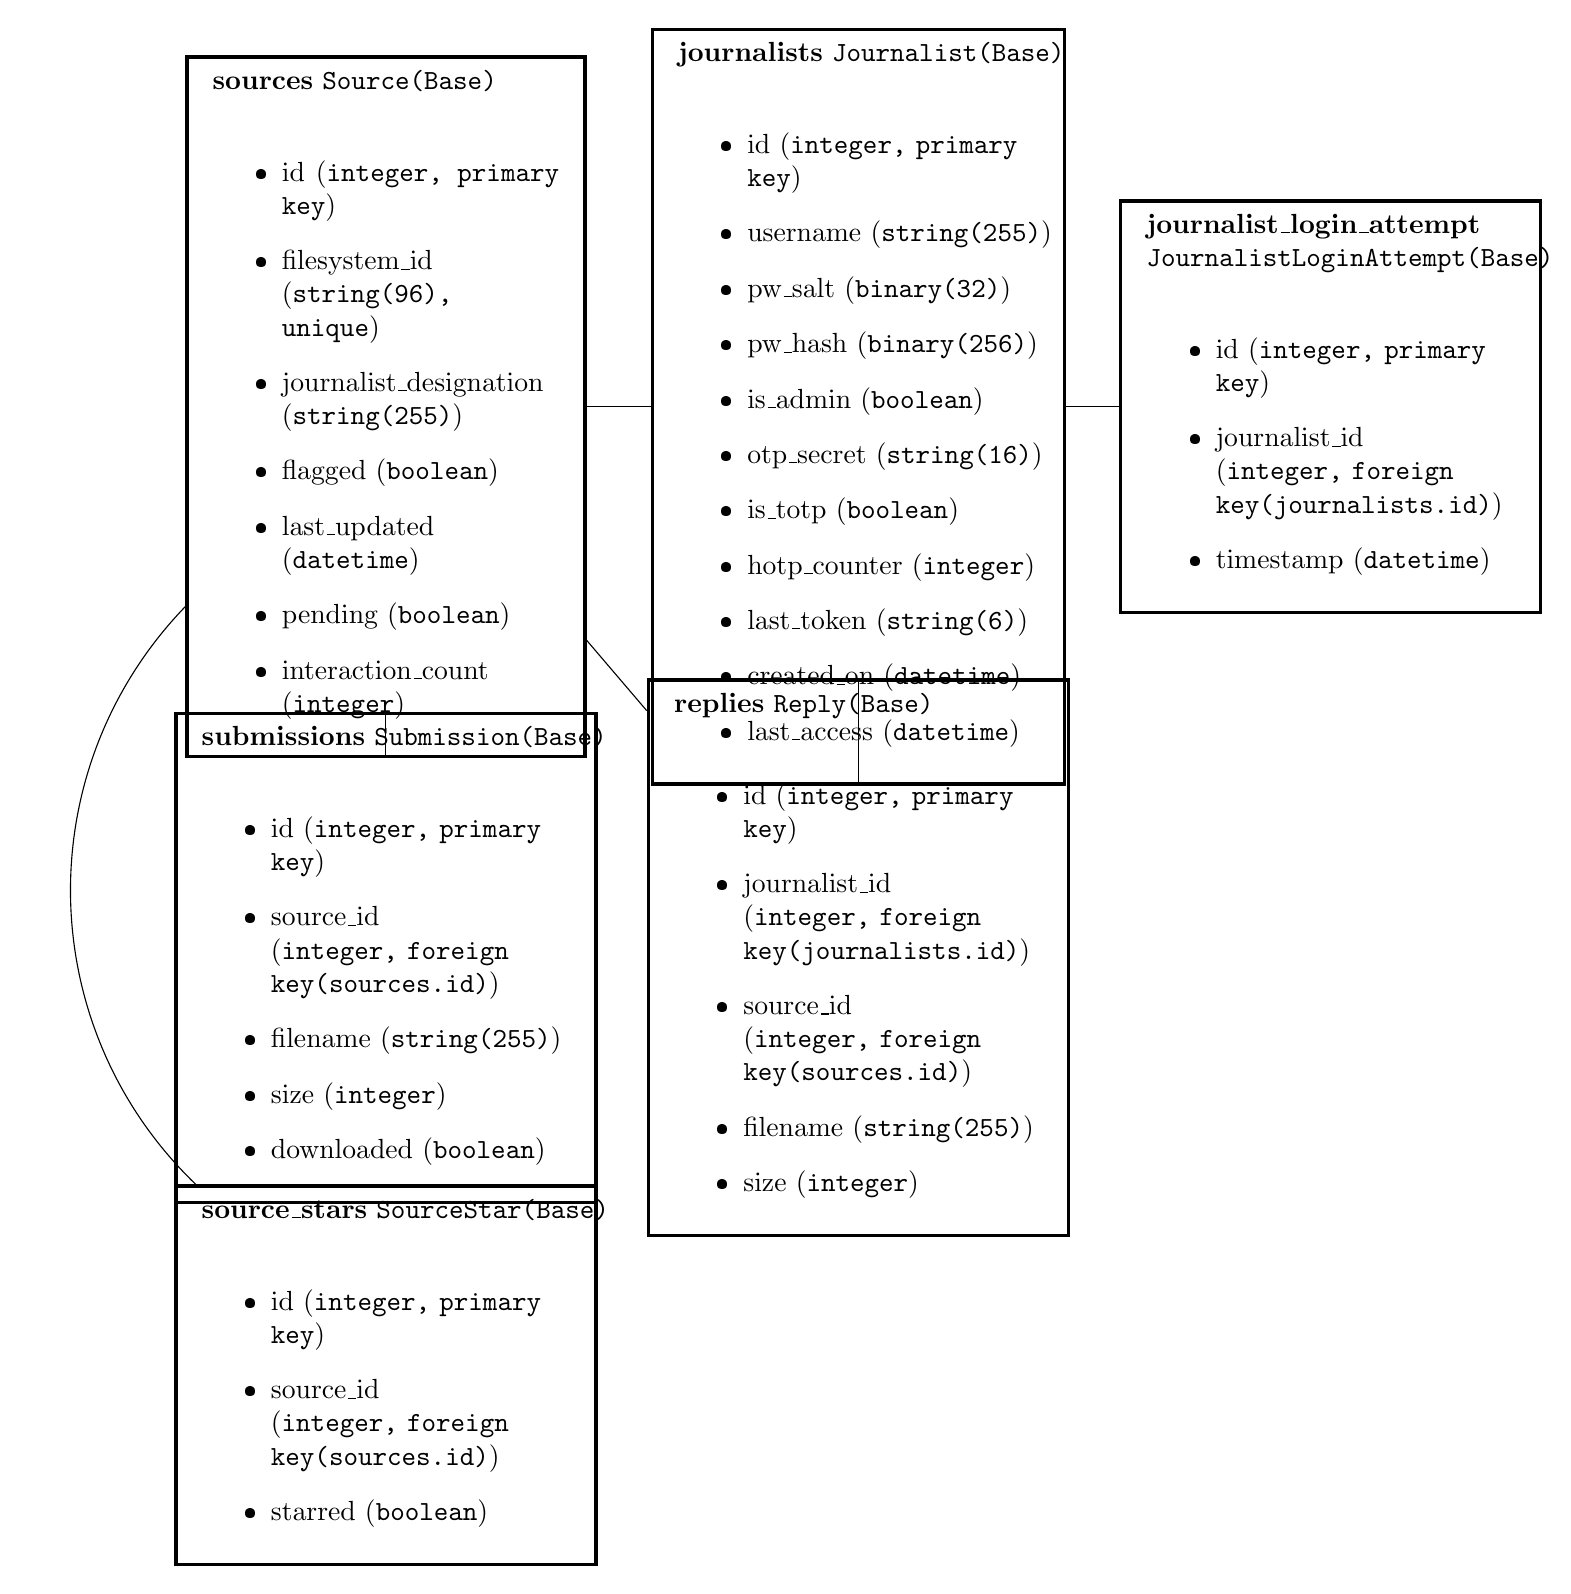
\begin{tikzpicture}[rotate=90]

 \node[state] (SOURCES) 
 {\begin{tabular}{l}
  \textbf{sources} \texttt{Source(Base)}\\\\
  \parbox{4.4cm}{\begin{itemize}
   \item id (\texttt{integer, primary key})
   \item filesystem\_id (\texttt{string(96), unique})
   \item journalist\_designation (\texttt{string(255)})
   \item flagged (\texttt{boolean})
   \item last\_updated (\texttt{datetime})
   \item pending (\texttt{boolean})
   \item interaction\_count (\texttt{integer})
  \end{itemize}
  }\\[4em]
 \end{tabular}};

 \node[state,
 right of=SOURCES,
 node distance=6cm,
 text width=5cm] (JOURNALISTS) 
 {\begin{tabular}{l}
  \textbf{journalists} \texttt{Journalist(Base)}\\ \\
  \parbox{5cm}{\begin{itemize}
   \item id (\texttt{integer, primary key})
   \item username (\texttt{string(255)})
   \item pw\_salt (\texttt{binary(32)})
   \item pw\_hash (\texttt{binary(256)})
   \item is\_admin (\texttt{boolean})
   \item otp\_secret (\texttt{string(16)})
   \item is\_totp (\texttt{boolean})
   \item hotp\_counter (\texttt{integer})
   \item last\_token (\texttt{string(6)})
   \item created\_on (\texttt{datetime})
   \item last\_access (\texttt{datetime})
  \end{itemize}
  }\\[4em]
 \end{tabular}};

 \node[state,
 right of=JOURNALISTS,
 node distance=6cm,
 text width=5.1cm] (JOURNALISTLOGINATTEMPTS) 
 {\begin{tabular}{l}
  \textbf{journalist\_login\_attempt} \\
  \texttt{JournalistLoginAttempt(Base)}\\ \\
  \parbox{5cm}{\begin{itemize}
   \item id (\texttt{integer, primary key})
   \item journalist\_id (\texttt{integer, foreign key(journalists.id)})
   \item timestamp (\texttt{datetime})
  \end{itemize}
  }\\[1em]
 \end{tabular}};
 
 \node[state,
 below of=SOURCES,
 node distance=7cm,
 text width=5.1cm] (SUBMISSIONS) 
 {\begin{tabular}{l}
  \textbf{submissions} \texttt{Submission(Base)}\\ \\
  \parbox{5cm}{\begin{itemize}
   \item id (\texttt{integer, primary key})
   \item source\_id (\texttt{integer, foreign key(sources.id)})   
   \item filename (\texttt{string(255)})
   \item size (\texttt{integer})
   \item downloaded (\texttt{boolean})
  \end{itemize}
  }\\[1em]
 \end{tabular}};

 \node[state,
 below of=SUBMISSIONS,
 node distance=5.3cm,
 text width=5.1cm] (SOURCESTAR) 
 {\begin{tabular}{l}
  \textbf{source\_stars} \texttt{SourceStar(Base)}\\ \\
  \parbox{5cm}{\begin{itemize}
   \item id (\texttt{integer, primary key})
   \item source\_id (\texttt{integer, foreign key(sources.id)})
   \item starred (\texttt{boolean})
  \end{itemize}
  }\\[1em]
 \end{tabular}};

 \node[state,
 below of=JOURNALISTS,
 node distance=7cm,
 text width=5.1cm] (REPLIES) 
 {\begin{tabular}{l}
  \textbf{replies} \texttt{Reply(Base)}\\ \\
  \parbox{5cm}{\begin{itemize}
   \item id (\texttt{integer, primary key})
   \item journalist\_id (\texttt{integer, foreign key(journalists.id)})
   \item source\_id (\texttt{integer, foreign key(sources.id)})
   \item filename (\texttt{string(255)})
   \item size (\texttt{integer})
  \end{itemize}
  }\\[4em]
 \end{tabular}};

 \path 
 (SOURCES) edge (JOURNALISTS)
 (JOURNALISTS) edge    (JOURNALISTLOGINATTEMPTS)
 (SOURCES) edge[bend right=45]  (SOURCESTAR)
 (SOURCES) edge (SUBMISSIONS)
 (REPLIES) edge (SOURCES)
 (REPLIES) edge (JOURNALISTS);

\end{tikzpicture}

\end{document}